\section{电路原理图}
\begin{figure}[H]
    \centering
    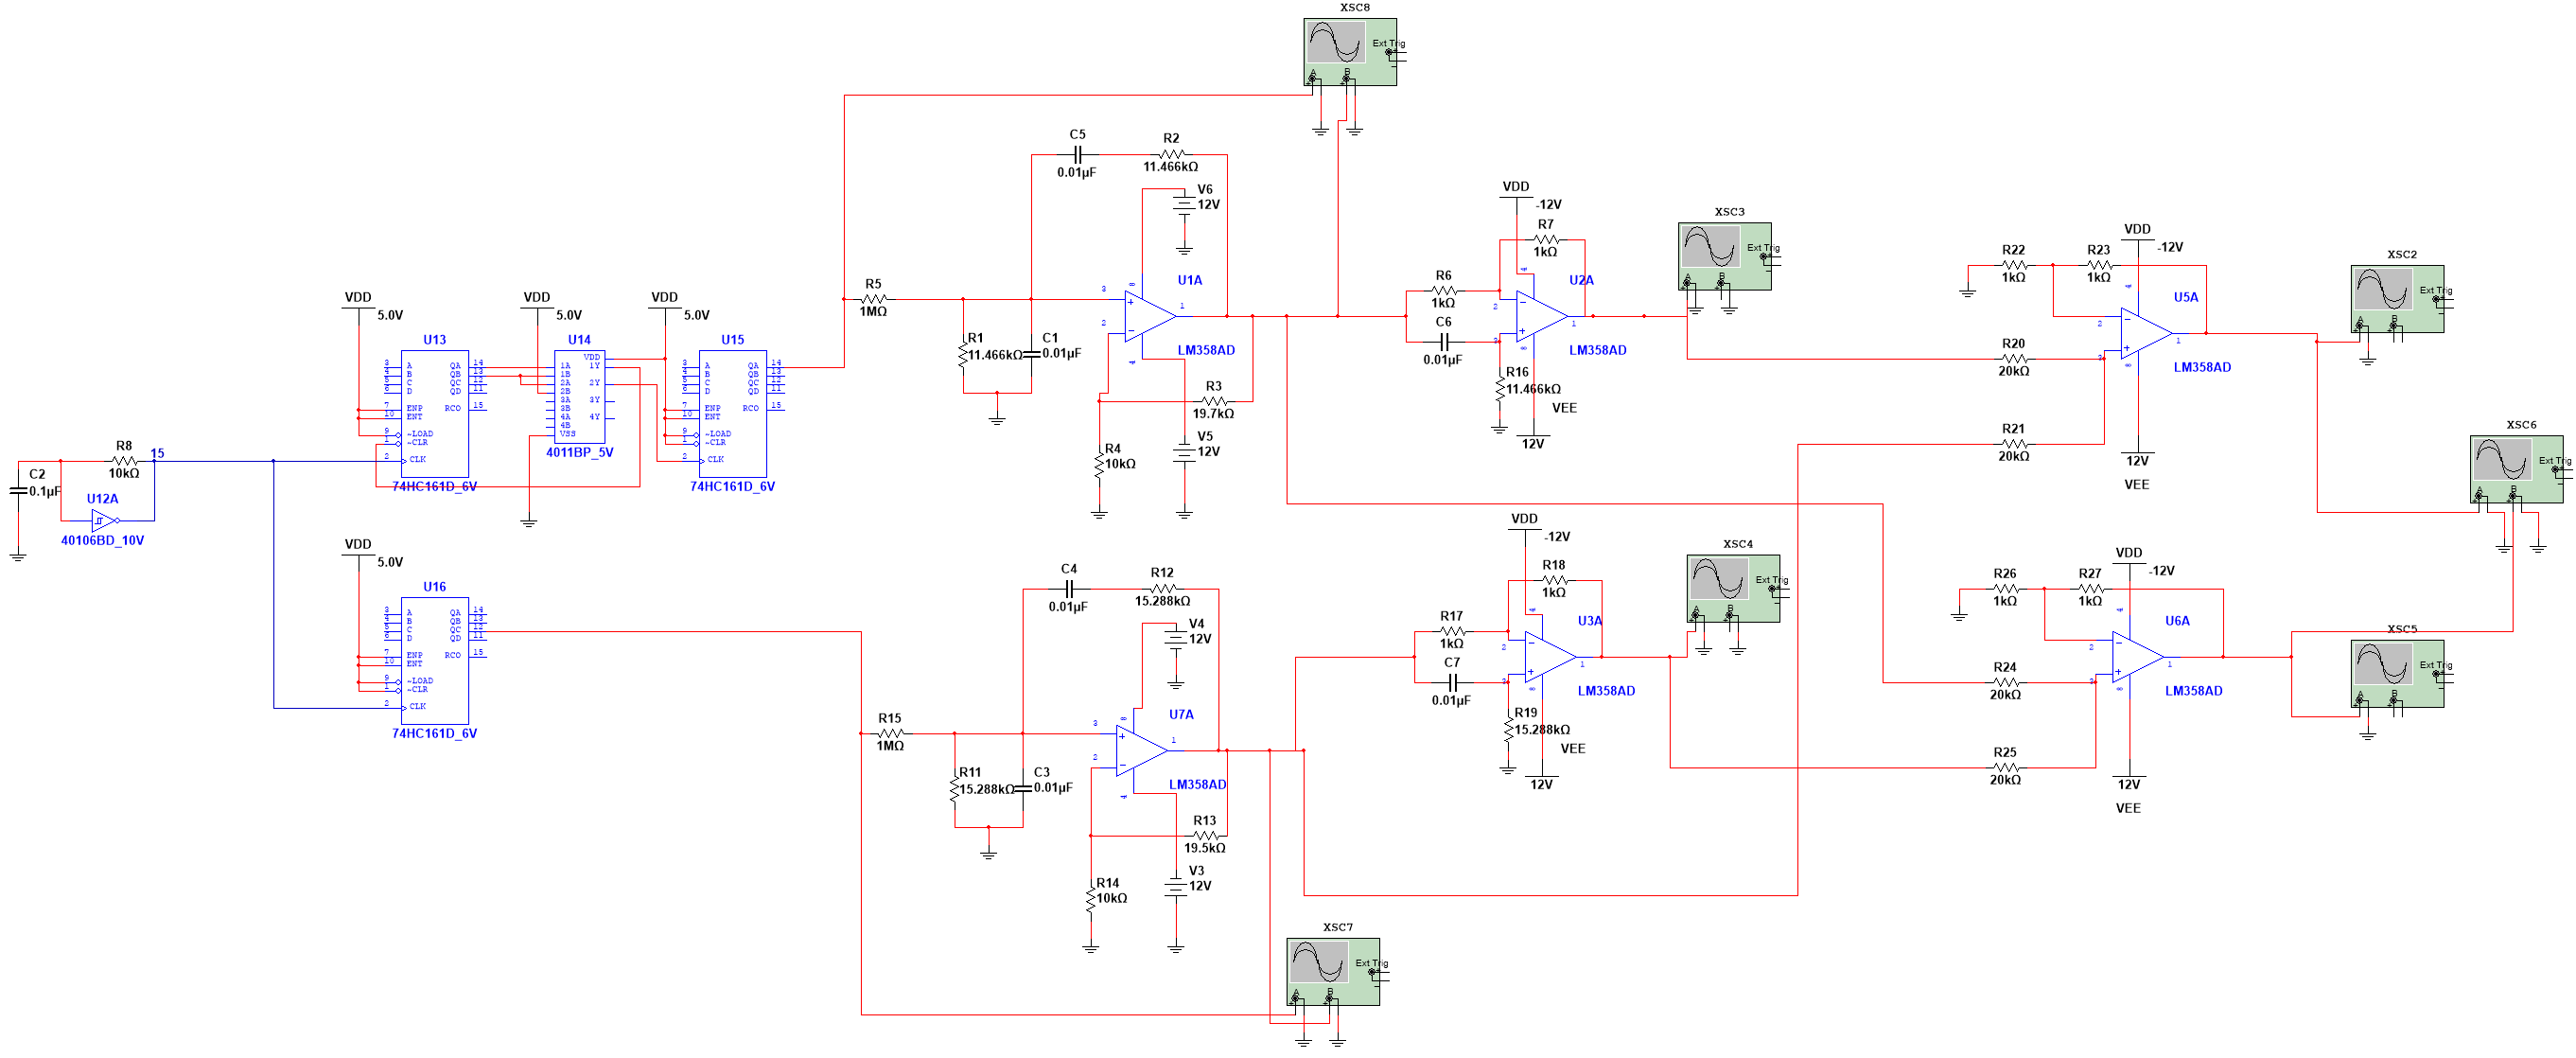
\includegraphics[width=1.2\linewidth,angle=-90]{images/circuit-full.png}
    \caption{电路原理图}
\end{figure}
多使用了一块面包板和一个74HC161芯片。



\section{示波器上呈现效果照片}
\begin{figure}[H]
    \centering
    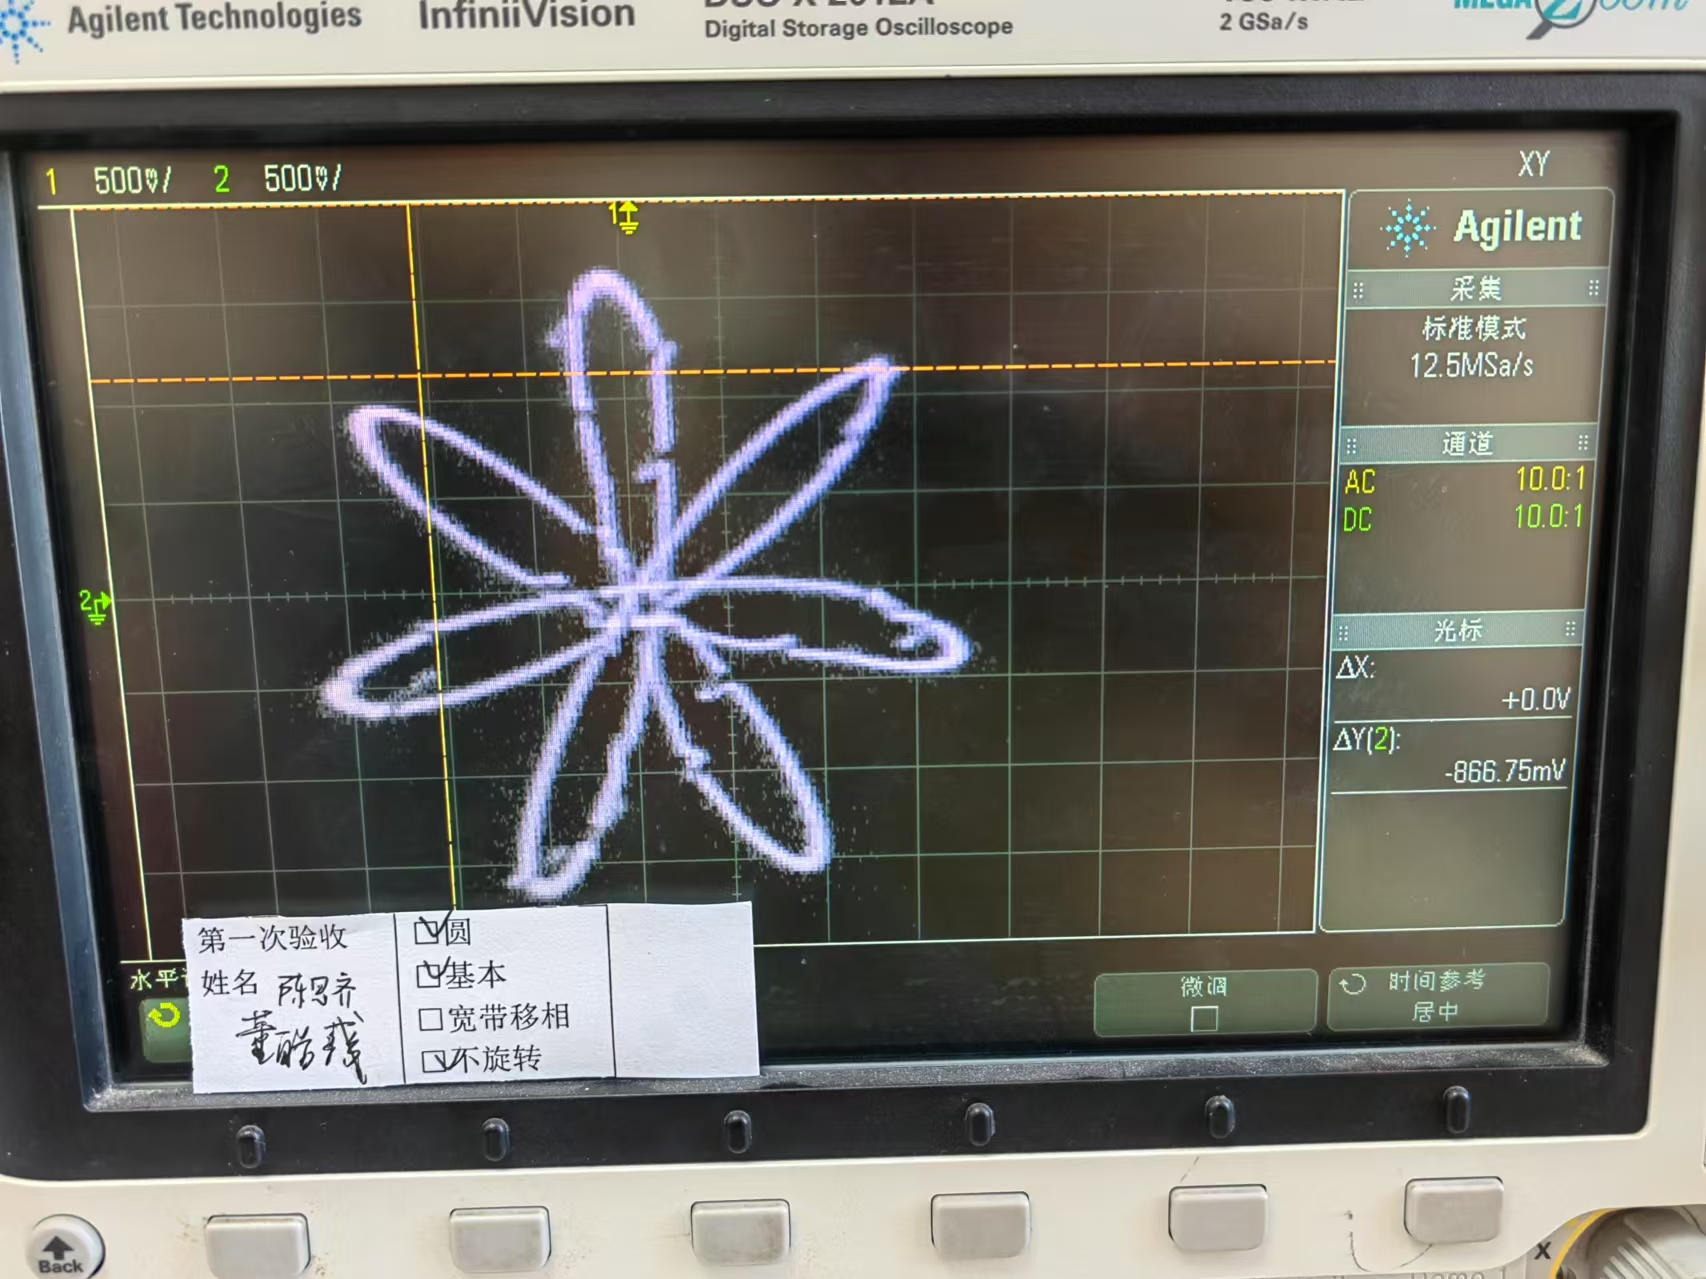
\includegraphics[width=0.6\linewidth]{images/result.jpg}
    \caption{最终万花尺图案}
\end{figure}
我们也尝试了其他的频率比(2:3),也得到了相应的图案。
\begin{figure}[H]
    \centering
    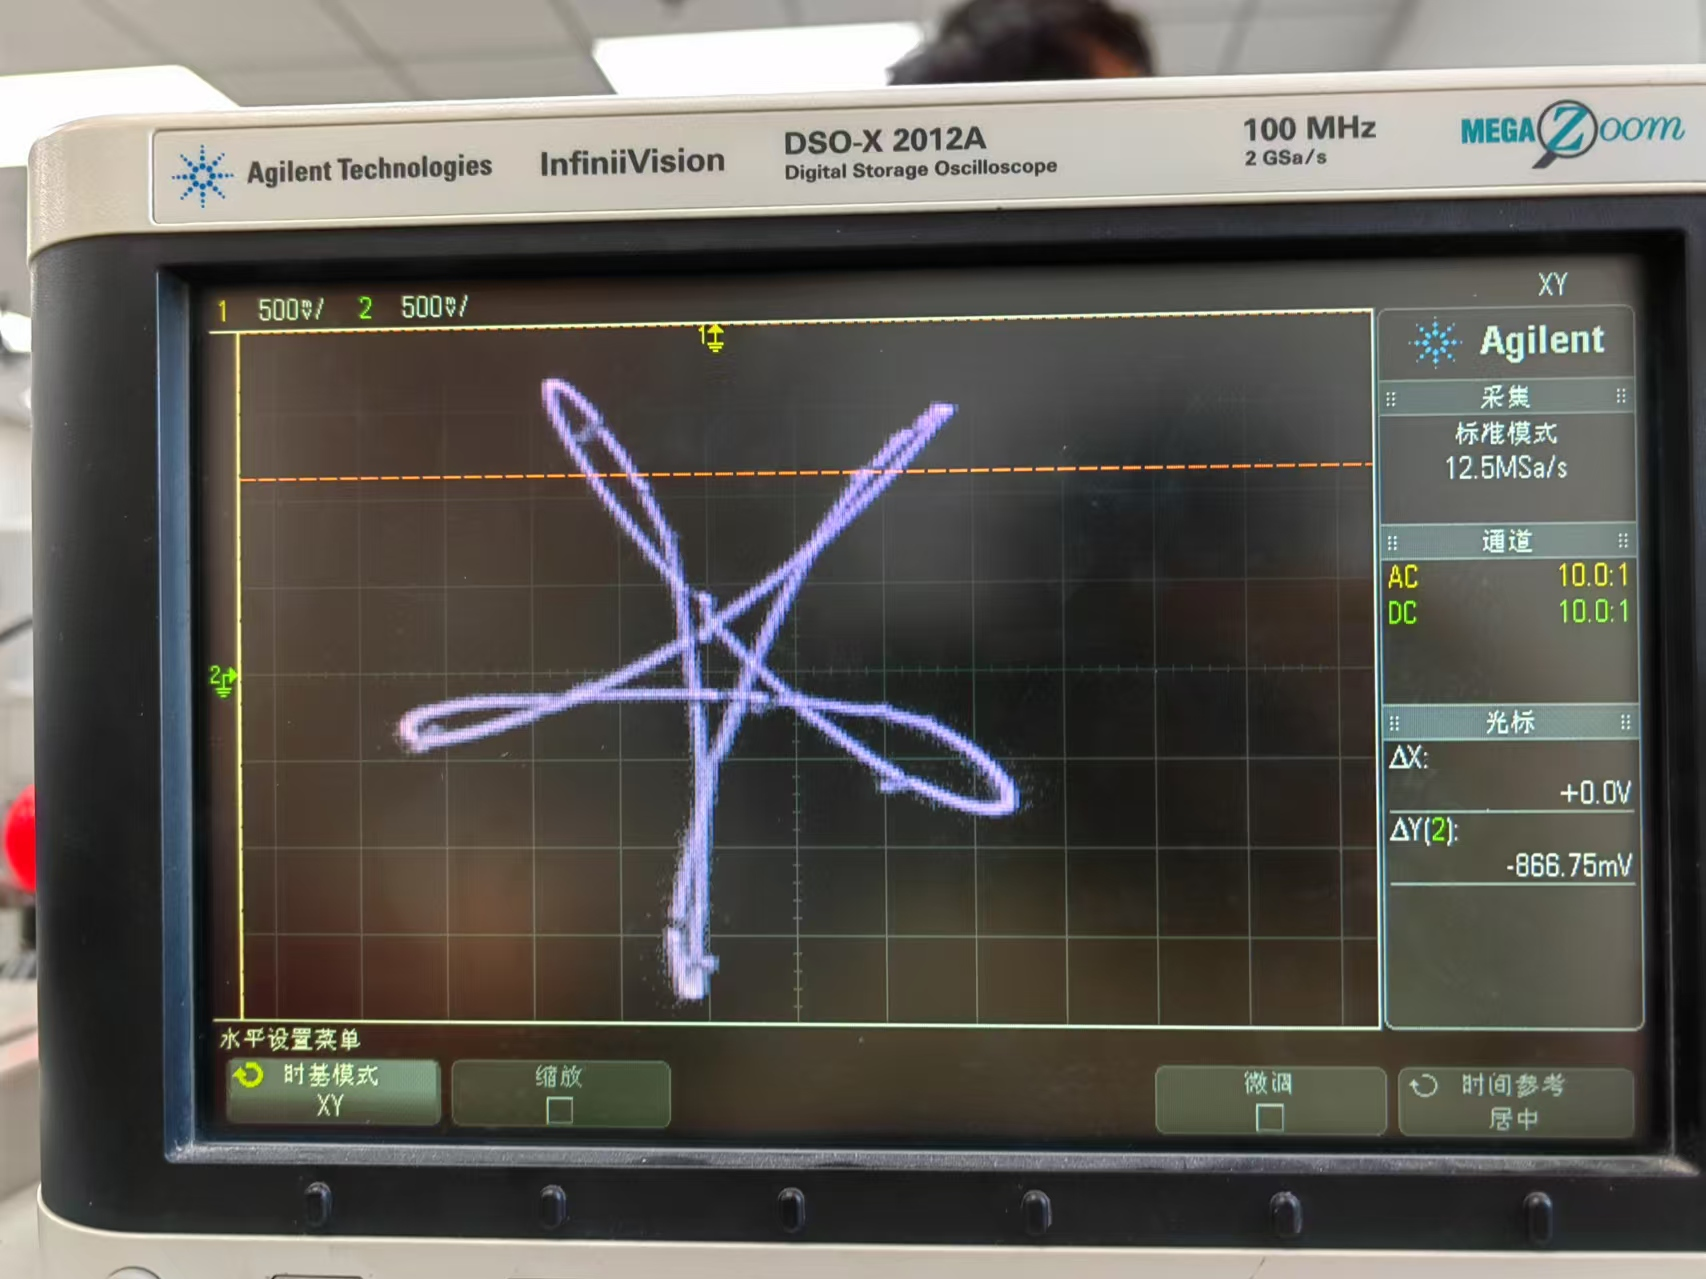
\includegraphics[width=0.6\linewidth]{images/result2.jpg}
    \caption{另一种万花尺图案}
\end{figure}



\section{电路整体照片}
\begin{figure}[H]
    \centering
    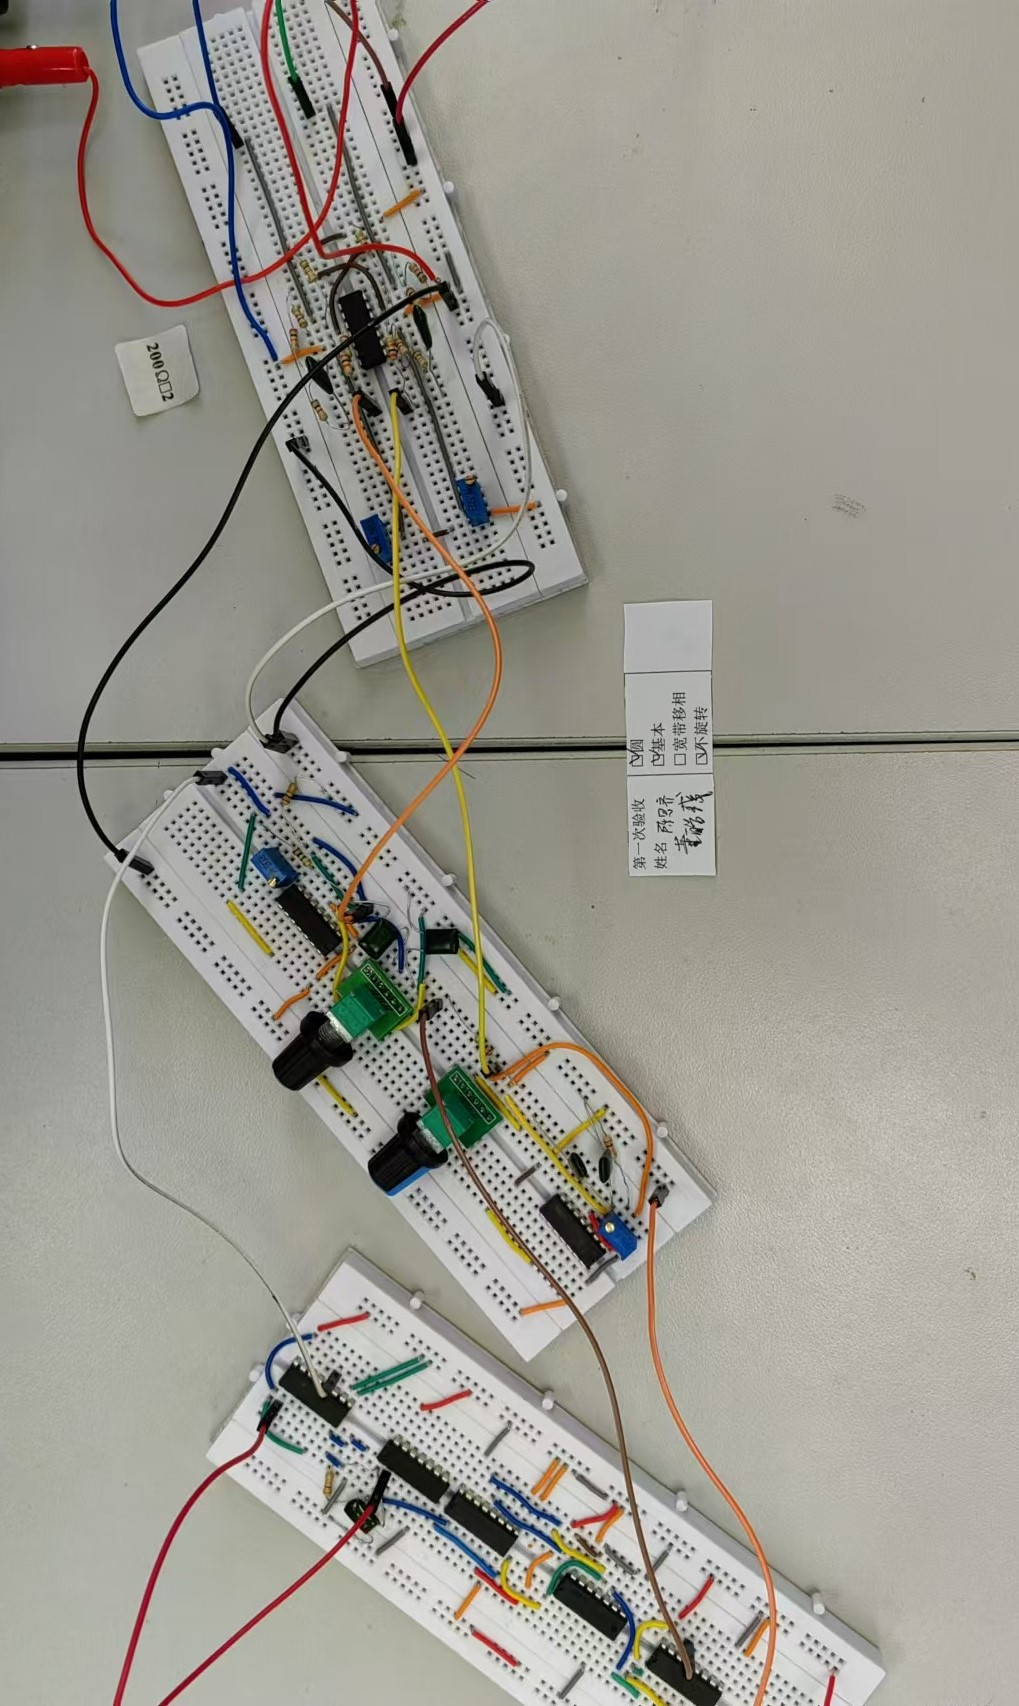
\includegraphics[width=0.7\linewidth]{images/circuit-real.jpg}
    \caption{实际电路图}
\end{figure}